% =============================================================================
\documentclass{beamer}
% \documentclass[draft]{beamer}
\usepackage{_style}
\usepackage{__config}

% The key part to use my theme
\usetheme{Falkor}

% Not integrated in my theme as not everybody wants that
\AtBeginSection[]
{
  \frame{
    \frametitle{Summary}
    {\scriptsize\tableofcontents[currentsection]}
  }
}

%%%%%%%%%%%%%%%%%%%%%%%%%%%% Header %%%%%%%%%%%%%%%%%%%%%%%%%%%%%%
\title{SC-Camp 2015}
\subtitle{Introduction to R and Data Analysis}

\author{\authors}
\institute[UL]{
  University of Luxembourg, Luxembourg
}

% Mandatory to define a logo - otherwise compilation will fail in an unobvious
% manner.
\pgfdeclareimage[height=0.8cm]{logo}{images/logo_UL.pdf}
\logo{\pgfuseimage{logo}}
\date{}

%%%%%%%%%%%%%%%%%%%%%%%%%%%%%% Body %%%%%%%%%%%%%%%%%%%%%%%%%%%%%%%
\begin{document}

\begin{frame}
    \vspace{2.5em}
    \titlepage
\end{frame}

% ......
\frame{
  \frametitle{Summary}
  {\scriptsize
    \tableofcontents
  }
}


%%%%%%%%%%%%%%%%%%%%%%%%%%%%%% Main Talk %%%%%%%%%%%%%%%%%%%%%%%%%%%%%%%
\section{Introduction to R}

\begin{frame}{R?}

R (pronounced aRrgh -- pirate style) is a programming language and
environment for statistical computing and graphics

\begin{itemize}
\item
  oriented towards data handling analysis and storage facility
\item
  R Base
\item
  Packages tools and functions (user contributed)
\item
  R Base and most R packages are available from the
  \href{cran.r-project.org}{Comprehensive R Archive Network (CRAN)}
\item
  Use R console or IDE: \textbf{Rstudio}, Deducer, vim/emacs\ldots{}
\item
  Comment is \textbf{\#}, help is \textbf{?} before a function name
\end{itemize}

\end{frame}

\begin{frame}[fragile]{Using R}

\begin{block}{\textbf{Installing/using packages}}

Install and load the \texttt{ggplot2} package (even if already
installed)

\begin{verbatim}
install.packages("ggplot2")
library(ggplot2)
\end{verbatim}

Or in one step, install if not available then load:

\begin{verbatim}
require(ggplot2) || {install.packages("ggplot2");
                     require(ggplot2)}
\end{verbatim}

\end{block}

\end{frame}

\begin{frame}{Using R}

\begin{block}{\textbf{Usefull Functions}}

\begin{itemize}
\item
  List all objects in memory: \texttt{ls()}
\item
  Save an object: \texttt{save(obj,\ file)}
\item
  Load an object: \texttt{load(file)}
\item
  Set working directory: \texttt{setwd(dir)}
\end{itemize}

\end{block}

\end{frame}

\begin{frame}{Data Structures}

\begin{itemize}
\item
  scalar:

  s = 3.14
\item
  vector:

  v = c(1, 2, ``ron'')
\item
  list:

  l = list(1:10, `a', pi)
\item
  matrix:

  m = matrix(seq(1:6), 2)
\item
  \textbf{dataframe}:

  df = data.frame(``col1'' = seq(1:4), ``col2'' = c(5, 6, ``cerveza'',
  6*7))
\item
  \ldots{}
\end{itemize}

\end{frame}

\begin{frame}[fragile]{Entering Data}

\begin{block}{Reading CSV or text files}

\begin{verbatim}
# comma separated values
dat.csv <- read.csv(<file or url>)
# tab separated values
dat.tab <- read.table(<file or url>, 
    header=TRUE, sep = "\t")
\end{verbatim}

\end{block}

\end{frame}

\begin{frame}[fragile]{Entering Data}

\begin{block}{Reading data from other software: Excel, SPSS\ldots{}}

Excel Spreadsheets -- need \texttt{xlsx} package

\begin{verbatim}
read.xlsx()
\end{verbatim}

SPSS and Stata both need the \texttt{foreign} package

\begin{verbatim}
dat.spss <- read.spss(<file or url>, 
                      to.data.frame=TRUE)
             
dat.dta <- read.dta(<file or url>)
\end{verbatim}

\end{block}

\end{frame}

\begin{frame}{Data Frames}

Most easy structure to use, have a matrix structure.

\begin{itemize}
\item
  \textbf{Observations} are arranged as \textbf{rows} and
  \textbf{variables}, either numerical or categorical, are arranged as
  \textbf{columns}.
\item
  Individual rows, columns, and cells in a data frame can be accessed
  through many methods of indexing.
\item
  We most commonly use \textbf{object{[}row,column{]}} notation.
\end{itemize}

\end{frame}

\begin{frame}[fragile]{Accessing Items in a \texttt{data.frame}}

Aside with R are provided example datasets, i.e. \texttt{mtcars} that
can be used

\begin{verbatim}
data(mtcars)
head(mtcars)
colnames(mtcars)

# single cell value
mtcars[2,3]
# omitting row value implies all rows
mtcars[,3]
# omitting column values implies all columns
mtcars[2,]
\end{verbatim}

\end{frame}

\begin{frame}[fragile]{Accessing Items in a \texttt{data.frame}}

We can also access variables directly by using their names, either with
\textbf{object{[},``variable''{]}} notation or \textbf{object\$variable}
notation.

\begin{verbatim}
# get first 10 rows of variable `mpg` using two methods:
mtcars[1:10, "mpg"]
mtcars$mpg[1:10]
\end{verbatim}

\end{frame}

\begin{frame}{Exploring Data}

\begin{block}{Description Of Dataset}

\begin{itemize}
\item
  Using \textbf{dim}, we get the number of observations(rows) and
  variables(columns) in the dataset.
\item
  Using \textbf{str}, we get the structure of the dataset, including the
  class(type) of all variables.

  dim(mtcars) str(mtcars)
\item
  \textbf{summary} when used on a dataset, returns distributional
  summaries of variables in the dataset.

  summary(mtcars)
\item
  \textbf{quantile} function enables to get statistical metrics on the
  selected data

  quantile(mtcars\$mpg)
\end{itemize}

\end{block}

\end{frame}

\begin{frame}{Exploring Data}

\begin{block}{Conditional Exploration}

\begin{itemize}
\item
  \textbf{subset} enables to explore data conditionally

  subset(mtcars, cyl \textless{}= 5)
\item
  \textbf{by} enables to call a particular function to sub-groups of
  data

  by(mtcars, mtcars\$cyl, summary)
\end{itemize}

\end{block}

\end{frame}

\section{Crazy Examples}\label{crazy-examples}

\begin{frame}[fragile]{Random Text Generation}

\begin{verbatim}
library(XML)
stem <- "http://www.5novels.com/classics/u5688"
hobbit <- NULL
for(i in 1:74) {
    if(i==1) { url <- paste0(stem, ".html") } 
    else { url <- paste0(stem, "_", i, ".html") }
    x <- htmlTreeParse(url, useInternalNodes=TRUE)
    xx <- xpathApply(x, "//p", xmlValue)
    hobbit <- c(hobbit, gsub("\r", "", xx[-length(xx)]))
    Sys.sleep(0.5)
}
hobbit = paste(hobbit, collapse=' ')
\end{verbatim}

\end{frame}

\begin{frame}[fragile]{Random Text Generation -- 2}

\begin{verbatim}
library(ngram)
ng2 <- ngram(hobbit, n=2)

babble(ng2, 128, seed=987654)
\end{verbatim}

\end{frame}

\begin{frame}{PiRates}

\animategraphics[autoplay,loop,height=5cm]{1}{../../figures/arrr-}{2013}{2014}

\end{frame}



%%%%%%%%%%%%%%%%%%%%%%%%%%%%%% Practical Session %%%%%%%%%%%%%%%%%%%%%%%%%%%%%%%


\section{Practical Session}
% ===============================================
\subsection{Pre-requisites}

% .......
\begin{frame}[fragile]
    \frametitle{Install and Run R}
    \begin{enumerate}
      \item On your local machine:
		\begin{itemize}
			\item Find a release that fits your distribution\\ at CRAN Archive\hfill\myurl{http://cran.r-project.org/}
			\item Install and launch R-Studio\hfill\myurl{https://www.rstudio.com/}
		\end{itemize}
      \item On the cluster\\
       First connect to the cluster, then submit a job to run R.
        \begin{cmdline}
            \cmdlinelocal{ssh gaia-cluster}\\
            \cmdlinefrontend{oarsub -I -l core=1,walltime="00:30:00"}\\
            \cmdlinenode{module load lang/R/3.2.0-ictce-7.3.5-bare}\\
            \cmdlinenode{R}
        \end{cmdline}
        \item Install and Load a Package
            \begin{cmdline}
              \cmdlineR{install.packages("ggplot2")}\\
              \cmdlineR{library(ggplot2)}\\
            \end{cmdline}
    \end{enumerate}
\end{frame}

% ===============================================
\subsection{Objectives}

% ............
\frame{

  \frametitle{Objectives of this Practical Session}

  \begin{itemize}
    \item Being able to plot data
     \begin{itemize}
      \item histogram for data distribution
      \item plot in different colors from different data sources
     \end{itemize}
    \item Know some tips to organize your data
     \begin{itemize}
      \item aggregate a dataset by column and apply an aggregation function
      \item data.table package for binary search in datasets
      \item performance in R operations
     \end{itemize}     
    \item R in parallel
     \begin{itemize}
      \item on one machine
      \item on a cluster with socket communications
      \item MPI communications
     \end{itemize}
     
\end{itemize}      
}

\subsection{Practical Session Details}

% .......
\frame{
  \frametitle{Exercises}
    \begin{itemize}
      \item Start the tutorial \myurl{\TPghurl}
      \begin{itemize} 
	      \item Plot 2 graphs in section Simple Plotting
	      \item Answer 2 questions at the end of section Organizing your Data
	      \item Compare performance of aggregation operations w/wo parallelization
      \end{itemize}
      \item Plot a speedup graph
      \begin{itemize}
       \item with different number of cores and/or machines
       \item needs: ggplot, parallel R
      \end{itemize}
    \end{itemize}
}

\frame{

  \frametitle{After the Practical Session: Problems}
      \begin{itemize}
        \item regression models: example and exercise
        \item parallelization of K-means Clustering: example and exercise
      \end{itemize}
  
}

\frame{
  \frametitle{Simple Plotting}
  Movies Histogram:
    \begin{center}
       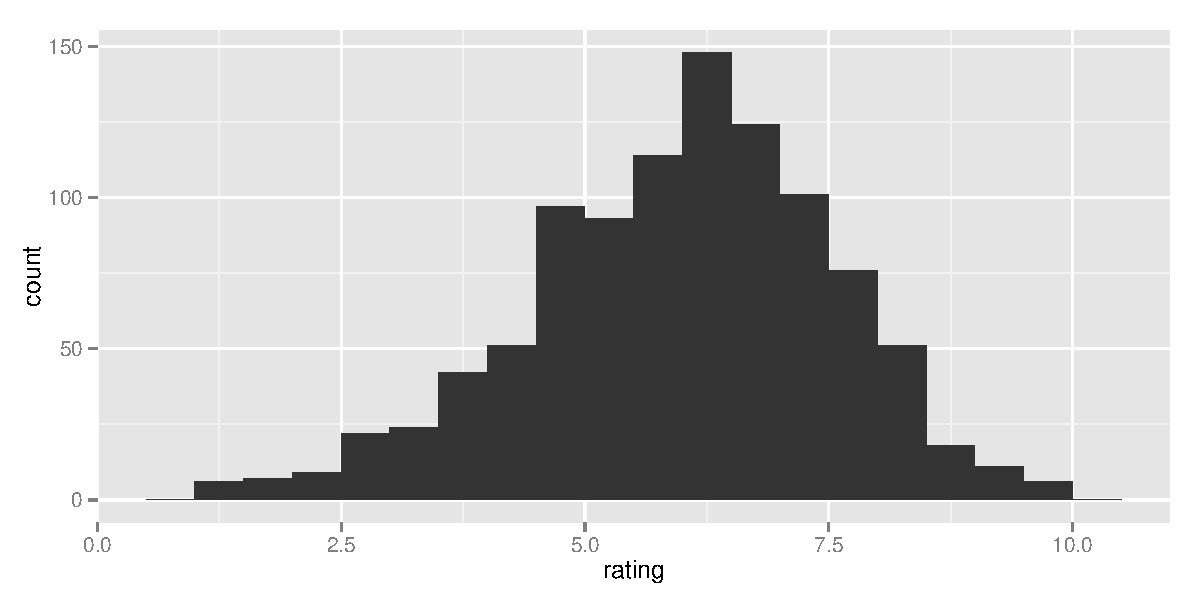
\includegraphics[scale=0.25]{figures/movies_hist.pdf}
    \end{center}
    
    Diamonds Plot with 2 colours:
    \begin{center}
       \hspace{1.8em}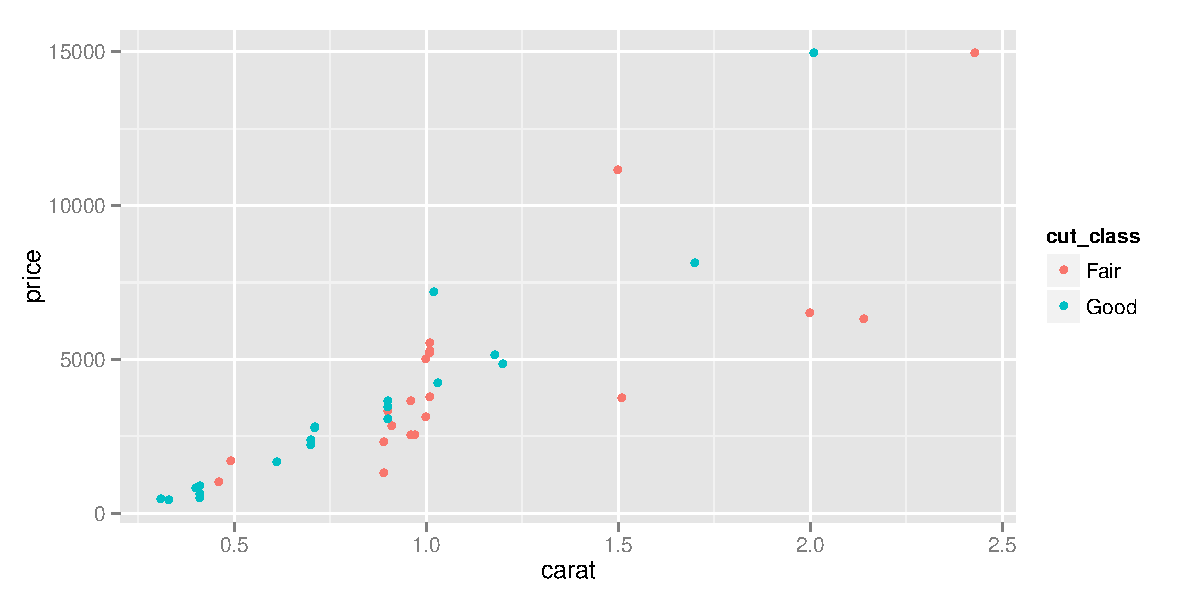
\includegraphics[scale=0.3]{figures/diamonds_plot.pdf}
    \end{center}
}

\frame[containsverbatim]{
  \frametitle{PS Questions}
  \begin{block}{Question: use ddply instead of tapply in the first example}
      \begin{lstlisting}[basicstyle=\tiny,numbers=none]
          ddply(DT, .(x), summarize, sum(v))
      \end{lstlisting}
  \end{block}   
  
  \begin{block}{Question: return the min and max instead of the sum.}
      \begin{lstlisting}[basicstyle=\tiny,numbers=none]
          min_max = function(data){
  			c(min(data), max(data))
		  }
          DT[,min_max(v),by=x]
          
          ## or  
                  
          DT[,c(min(v), max(v)),by=x]	
      \end{lstlisting}
  \end{block}  
}


\section*{Thank you for your attention...}
\frame{
  \frametitle{Questions?}
  \begin{center}
      
\includegraphics[scale=0.2]{question.jpg}
  \end{center}

  {\tiny
    \tableofcontents

  }
}

\newcounter{finalframe}
\setcounter{finalframe}{\value{framenumber}}

% \appendix

\frame{
  \frametitle{Usefull links}

    \begin{itemize}
      \item CRAN Archive \hfill\myurl{http://cran.r-project.org/}
      \item ggplot2 Documentation \hfill\myurl{http://docs.ggplot2.org/current/}
      \item CRAN HPC\\ Packages \hfill\myurl{http://cran.r-project.org/web/views/HighPerformanceComputing.html}
      \item Advanced R programming by Hadley Wickham \hfill\myurl{http://adv-r.had.co.nz/}
    \end{itemize}
}

\setcounter{framenumber}{\value{finalframe}}

\end{document}


% ~~~~~~~~~~~~~~~~~~~~~~~~~~~~~~~~~~~~~~~~~~~~~~~~~~~~~~~~~~~~~~~~
% eof
% 
% Local Variables:
% mode: latex
% mode: flyspell
% mode: visual-line
% TeX-master: "."
% End:
